\documentclass{article}

\usepackage[utf8]{inputenc}
\usepackage[T1]{fontenc}
\usepackage{textcomp}
\usepackage[italian]{babel}
\usepackage{graphicx}
\usepackage{siunitx}
\usepackage{hyperref}
\usepackage{float}
\usepackage{amsmath, amssymb}

\sisetup{uncertainty-mode=separate}

\title{Relazione di Laboratorio 1 - Lente cilindrica}
\author{Walhout Francesco e Iallorenzi Michele}

\begin{document}

\maketitle

\section{Introduzione}
    Questo esperimento consiste nel misurare la lunghezza focale di una lente cilindrica, che nel nostro caso sarà un comune bicchiere. Utilizzeremo degli strumenti che si possono trovare in casa e faremo un Fit con la Legge dei Punti Coniugati (\ref{eq:punti_coniugati}) e confronteremo il risultato sperimentale con il risultato teorico fornito dalla legge \ref{eq:lente_cilindrica}.



\section{Esperienza}

    \subsection{Strumenti}
    \begin{itemize}
        \item Bicchiere cilindrico (non troppo spesso)
        \item Smartphone o torcia elettrica
        \item Metro a nastro
        \item Schermo (si può utilizzare un qualunque oggetto, basta che sia piano e che raccolga l'immagine proiettata dal bicchiere)
    \end{itemize}

    \subsection{Misurazione}
    Disponiamo il bicchiere in una posizione a piacere (comoda per la misurazione) e versiamo nel bicchiere l'acqua. Cercando di mantenere il telefono e lo schermo paralleli, posizioniamoli ad una certa distanza dal bicchiere, lo schermo a una parte ed il cellulare dall'altra, poi accendiamo la torcia.
    Disponiamo lo schermo e la torcia in modo da formare una linea sottile (il più possibile) sullo schermo.
    Ora facciamo 7 misurazioni dove cerchiamo di ottenere sullo schermo una linea che sia sottile il più possibile; cambiamo la posizione del cellulare e dello schermo per 7 volte facendo la stessa procedura. Misuriamo queste coppie di distanze torcia-schermo, dopo aver fissato come origine del sistema di riferimento il centro della circonferenza alla base del bicchiere.\\
    Come incertezza di misura abbiamo scelto $\sigma_p = \sigma_q = \SI{3}{\mm}$ dato che, nonostante
    la risoluzione strumentale fosse di $\SI{1}{\mm}$, è difficile assicurarsi che lo schermo sia
    alla distanza corretta per formare un immagine perfettamente nitida.\\
    Ora che abbiamo preso i dati, passiamo all'elaborazione di questi ultimi.



\section{Elaborazione dei dati}
    Per qualsiasi lente sottile (ovvero una lente con spessore trascurabile)
    vale la seguente legge che mette in relazione le grandezze $p$, $q$ con la lunghezza
    focale $f$:
    \begin{equation}\label{eq:punti_coniugati}
        \frac{1}{p} + \frac{1}{q} = \frac{1}{f}
    \end{equation}
    Scriviamo un codice di Python che possa fare un Fit dei dati appena raccolti.
    Notiamo che è possibile linearizzare la legge \ref{eq:punti_coniugati},
    introducento le due variabili $x$ e $y$ (indipendente e dipendente) e facendo una sostituzione: $x = 1/p$ e $y = 1/q$.\\
    Si ottiene quindi:
    \begin{equation}\label{eq:relazione}
        y = -x +\frac{1}{f}
    \end{equation}
    In questo caso particolare, le incertezze sulla variabile x non sono trascurabili, quindi il fit dei minimi quadrati non si può applicare, e sarà necessario utilizzare l'algoritmo di orthogonal distance regression (ODR). Grazie a questo riusciremo a stimare il valore di $f$, che abbiamo ottenuto sperimentalmente.
    In particolare eseguiamo il fit lasciando libero il coefficiente angolare $m$, utilizzando quindi l'equazione 
    $y=mx+\frac{1}{f}$, il fit ed i dati sperimentali sono mostrati in figura \ref{fig:lente_cilindrica}.\\
    In questo caso ci torna:
    \begin{gather*}
        m = -1.1 \pm 0.1\\
        f = \SI{7.2\pm 0.4}{\cm}
    \end{gather*}
    \begin{figure}[ht!]
        \centering
        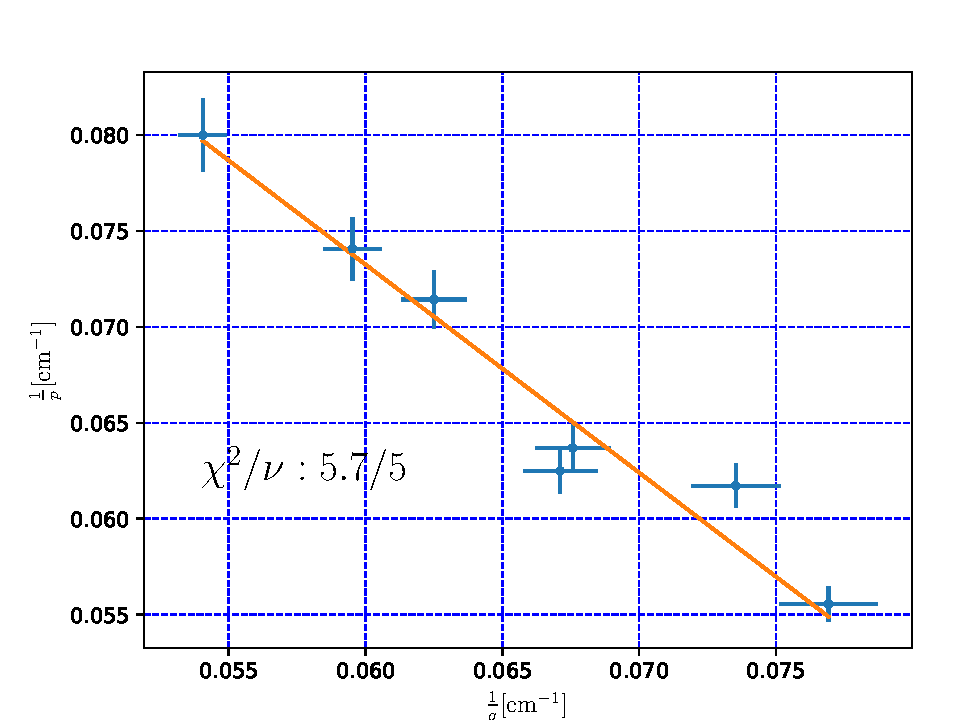
\includegraphics[width=0.8\textwidth]{extra/lente_cilindrica.pdf}
        \caption{Grafico della relazione \ref{eq:relazione}}
        \label{fig:lente_cilindrica}
    \end{figure}



\section{Analisi dati}
    Nella sezione precedente abbiamo ricavato i dati sull'esperimento attraverso il nostro codice di Python. Adesso utilizziamo una legge che ci dovrebbe dare, dal punto di vista teorico, la focale di una lente cilindrica, per poi confrontare il valore con la $f$ ottenuta prima.\\
    L'equazione che fa al caso nostro è la seguente:
    \begin{equation}\label{eq:lente_cilindrica}
        \frac{1}{f} = \frac{2}{r} (\frac{n-1}{n})
    \end{equation}
    Sapendo che l'indice di rifrazione $n$ è quello dell'acqua, ed avendo misurato il raggio del bicchiere, abbiamo ricavato questi dati:
    \begin{gather*}
        n_{acqua} = 1,33 \\
        r = \SI{3,75}{\cm} \\
        f = \SI{7,56}{\cm}
    \end{gather*}




\section{Conclusioni}
    Il fit ottenuto risulta soddisfacente e il valore sperimentale ottenuto
    per la lunghezza focale è in buon accordo con quello previsto dalla teoria.
    Possiamo quindi dirci soddisfatti di questa misura indiretta di $f$ e affermare che
    l'equazione \ref{eq:punti_coniugati} è un modello adeguato nelle condizioni in
    cui abbiamo svolto l'esperimento.

    
\end{document}
